The choice of rods to model the cable was done because it seemed to be the simpler
way to get a good cable behaviour.

\section{SimMechanics\texttrademark ~Multi-Body Engine}

In order to get a model quickly, the use of an easy to made model was done with SimMechanics in Simulink.
The program allow to easily connect parts and their joints.The SimMechanics engine will be handling the movement of the cable and the effect of forces on it.

\begin{figure}[H]
\centering
    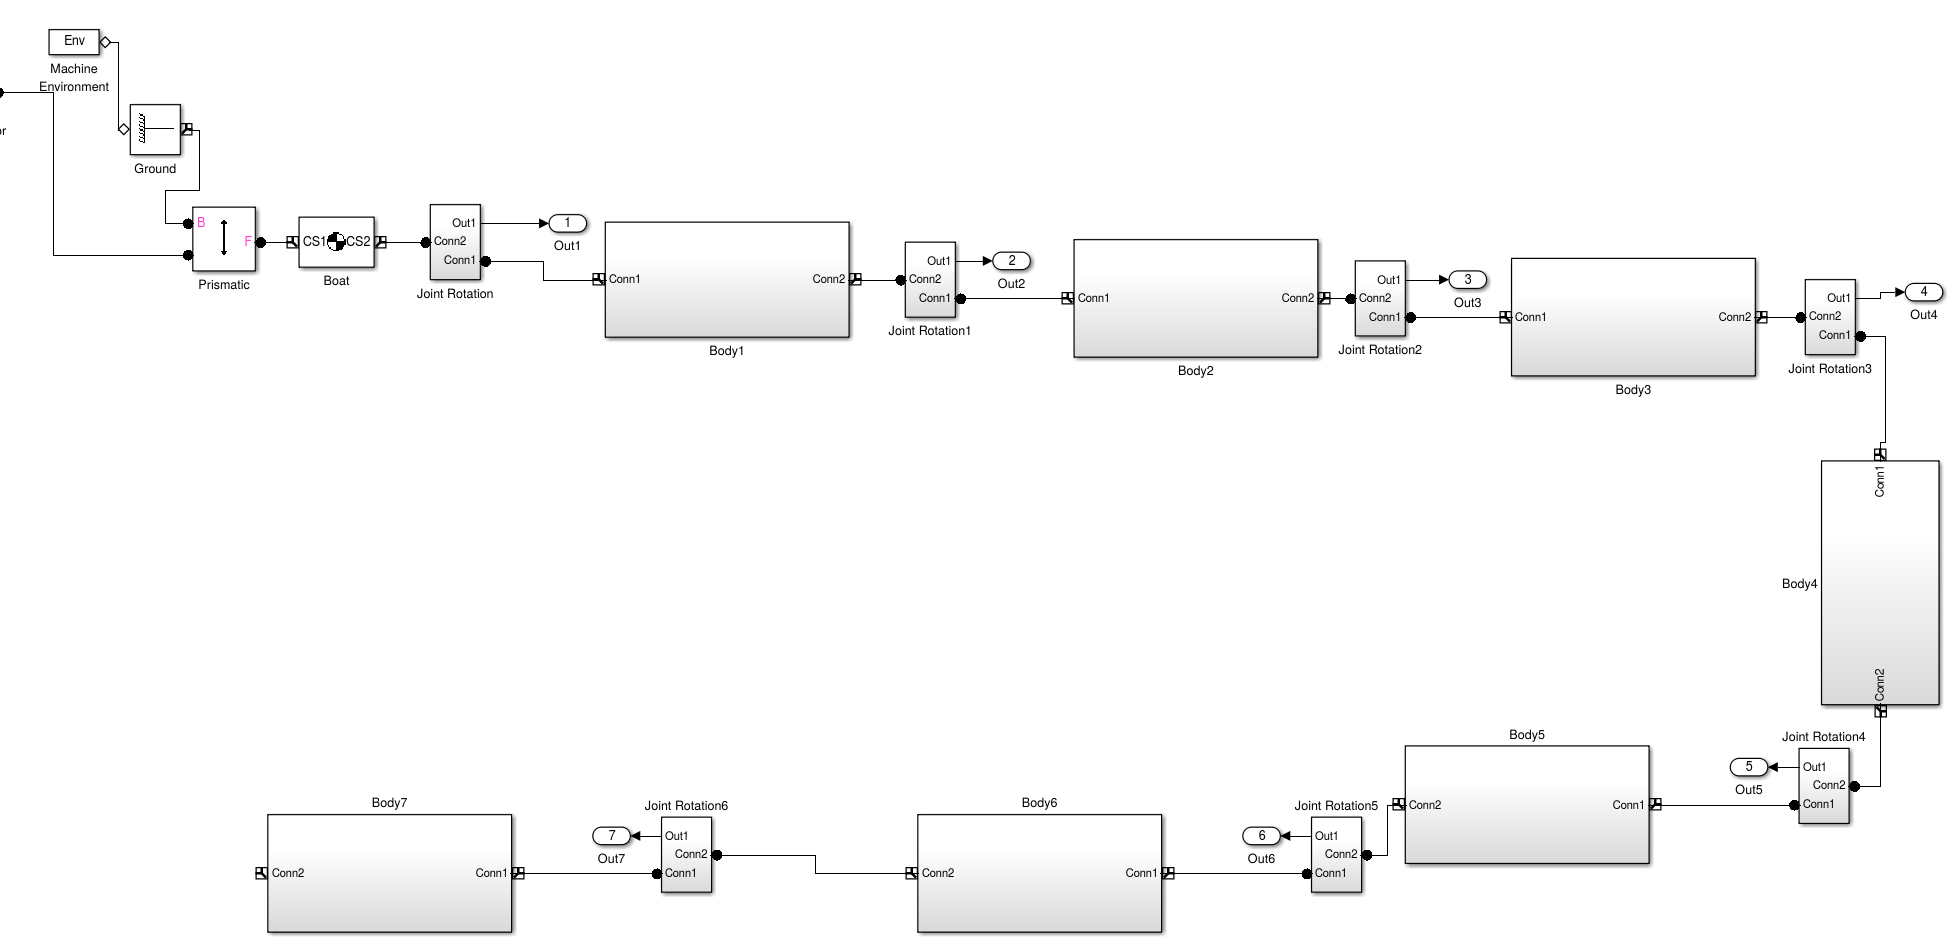
\includegraphics[scale=0.2,angle=0]{MultyBodySimMech.png}
    \caption{Simulink Model of the Cable.}
    \label{fig:SimulinkFullMod}
\end{figure}

The implementation of the model in Simulink is done in a graphic way (see~\ref{fig:SimulinkFullMod}). In
this first model the cable is modelled via seven rods connected via 2 degree of freedom joints, which are rotations.

\begin{figure}[H]
\centering
    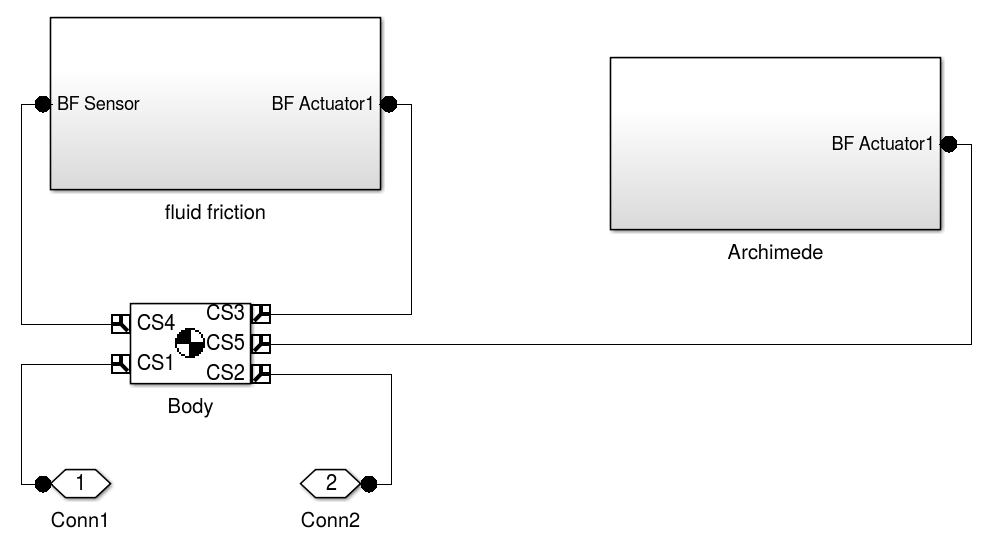
\includegraphics[scale=0.35,angle=0]{rod_pic.png}
    \caption{Single rod, a part of the cable.}
    \label{fig:SingleRod}
\end{figure}

Each rod is represented by a body, the object handled by SimMechanics, this body got a mass and an inertia matrix,here the inertia for a cylinder has been chosen. Then the application points of the forces and joints are
initialized.

The gravity is automatically computed by SimMechanics but not other optionals forces (at least for the first generation) such as the fluid friction and the Archimedes principle. 

\begin{figure}[H]
\centering
    \begin{minipage}[b]{0.4\textwidth}
    \centering
    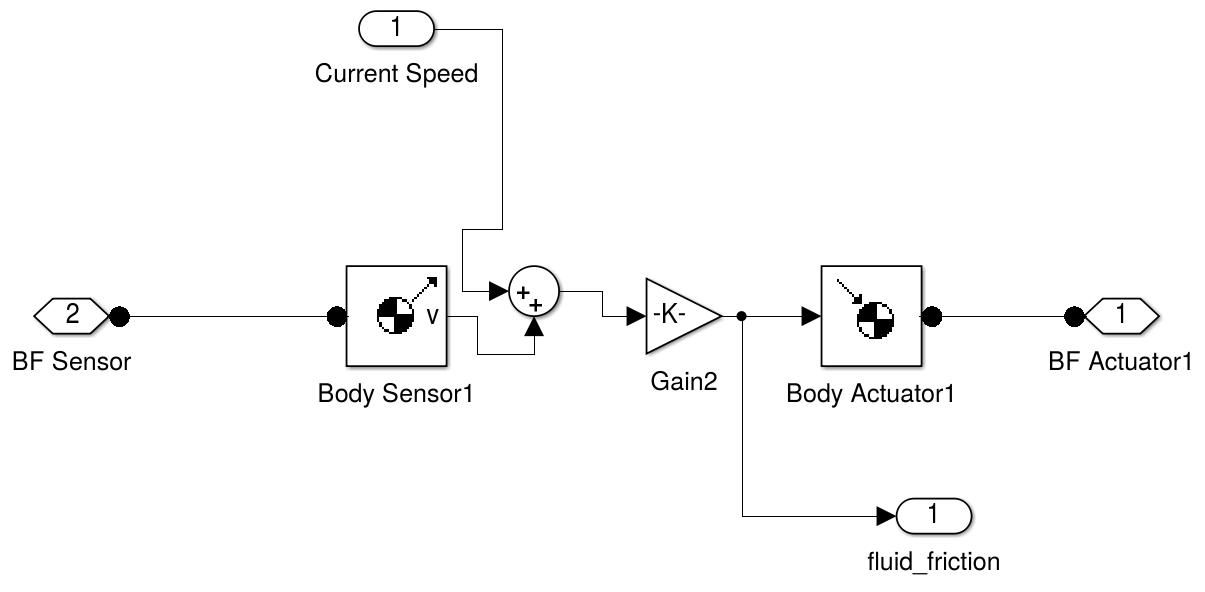
\includegraphics[scale=0.2,angle=0]{fluidfrictionSimMech.png}
    \caption{Computation of the fluid friction forces in Simulink.}
    \label{fig:fluidSimMech}
    \end{minipage}
    \hfill
    \begin{minipage}[b]{0.4\textwidth}
    \centering
    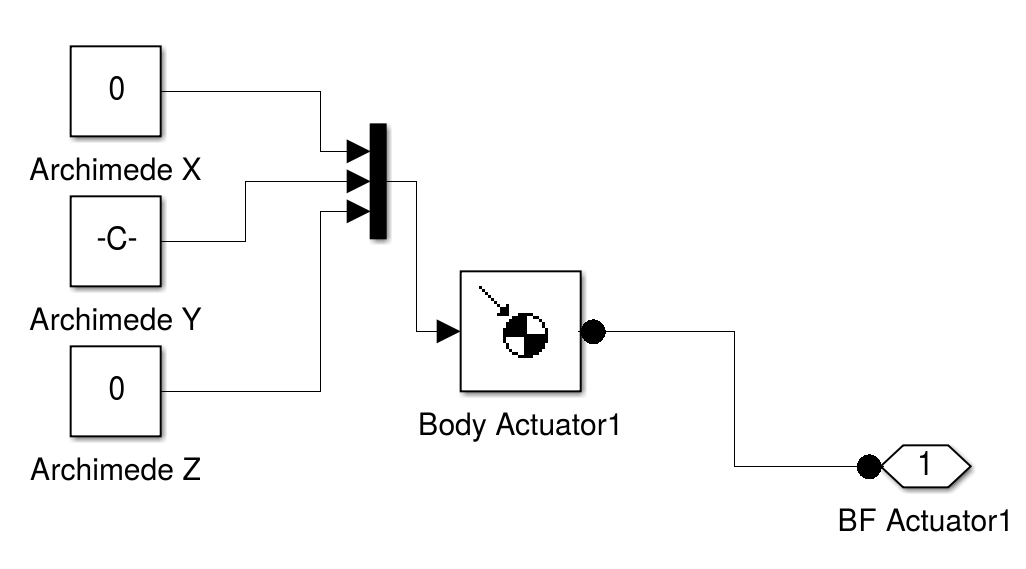
\includegraphics[scale=0.2,angle=0]{archiSimMech.png}
    \caption{Computation of the Archimedes force in Simulink.}
    \label{fig:archSimMech}
    \end{minipage}
\end{figure}

To compute the other forces SimMechanics allows the application of forces and torque on the body therefore, for each
body a sensor (see~\ref{fig:fluidSimMech}) output the velocity of the center of gravity of the rod, then the 
fluid friction is computed for each direction (the coefficient stay the same for each direction and pose of the cable in this model) to be applied on the body via an actuator \footnote{The video of the simulation can be see here \href{https://youtu.be/xEDApnU54ac}{Simulink video}.}.

\begin{figure}[H]
\centering
    \begin{minipage}[b]{0.5\textwidth}
    \centering
    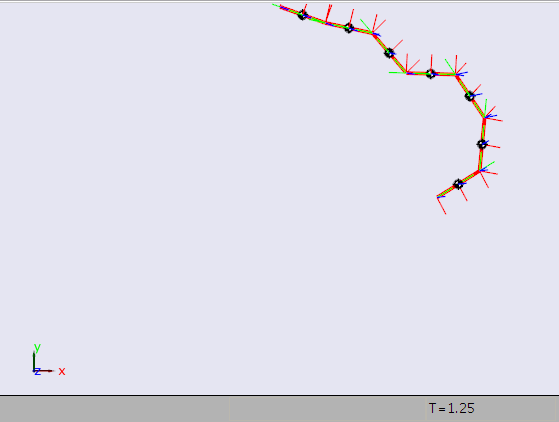
\includegraphics[scale=0.4,angle=0]{cable_simu2.png}
    \caption{Output of the Simulink simulation with random pose at the start.}
    \label{fig:Out1SimMech}
    \end{minipage}
    \hfill
    \begin{minipage}[b]{0.45\textwidth}
    \centering
    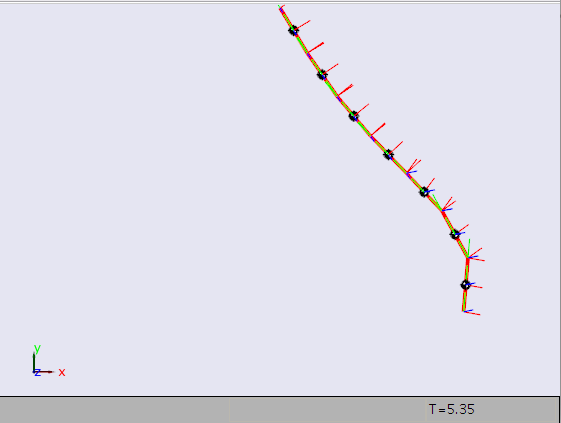
\includegraphics[scale=0.4,angle=0]{cable_simu1.png}
    \caption{Output of the Simulink simulation a few second later than~\ref{fig:Out1SimMech}.}
    \label{fig:Out2SimMech}
    \end{minipage}
\end{figure}


More simulation has been made to determine the behaviour of the cable, mainly the cable is attached on a point following a strict line with a constant speed, the cable is towed but has no action on the towing point for the moment.

\begin{figure}[H]
\centering
    \begin{minipage}[b]{0.4\textwidth}
    \centering
    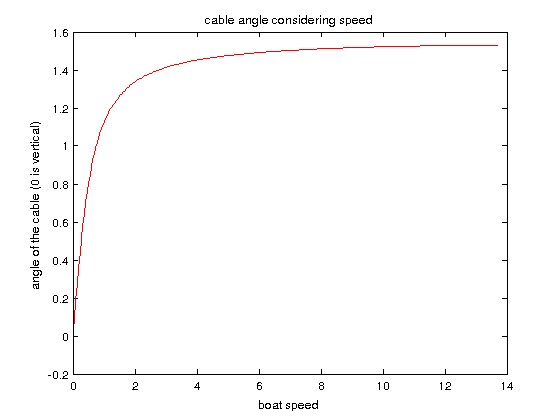
\includegraphics[scale=0.45,angle=0]{angle_over_speed_r.png}
    \caption{Angle of the cable to the vertical depending on the speed of the boat.}
    \label{fig:angleSpeed}
    \end{minipage}
    \hfill
    \begin{minipage}[b]{0.45\textwidth}
    \centering
    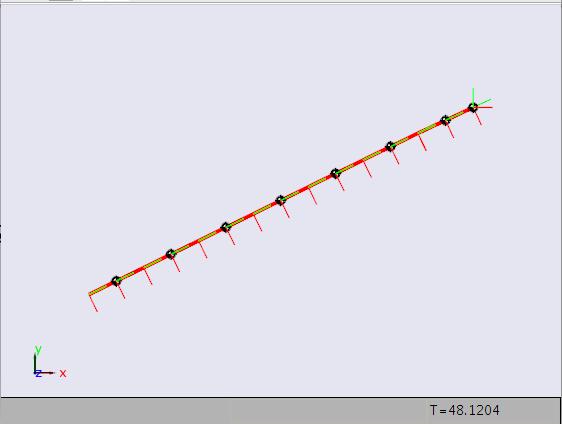
\includegraphics[scale=0.35,angle=0]{stabilized_cable.png}
    \caption{Output of a stabilized cable when towed by a particle with a constant and rectilinear motion.}
    \label{fig:stabCable}
    \end{minipage}
\end{figure}

In figure~\ref{fig:angleSpeed} is represented the angle of the cable to the vertical depending of the speed of the 
boat when the system is stabilized. The curve resemble to an inverse curve dependant on the density of the cable.
It means beyond a certain velocity the cable will be useless due to be not enough submerged.

\begin{figure}[H]
\centering
    \begin{minipage}[b]{0.4\textwidth}
    \centering
    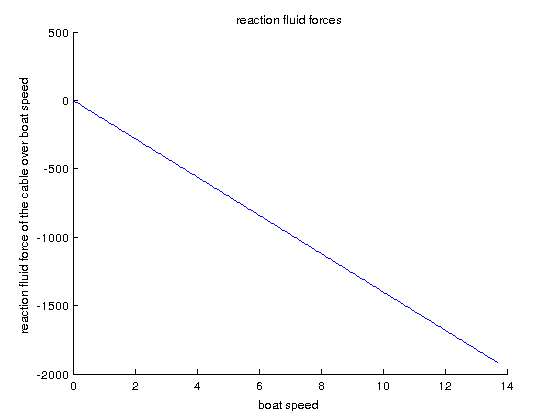
\includegraphics[scale=0.45,angle=0]{fluid_forces_over_speed.png}
    \caption{Resultant of the fluid forces when stabilized depending on the speed.}
    \label{fig:fluidSpeed}
    \end{minipage}
    \hfill
    \begin{minipage}[b]{0.45\textwidth}
    \centering
    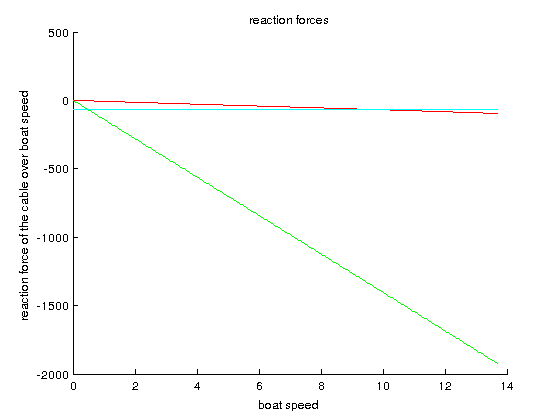
\includegraphics[scale=0.45,angle=0]{forces_over_speed_r.png}
    \caption{Resultant of forces on the joint boat-cable depending on the speed.}
    \label{fig:forceSpeed}
    \end{minipage}
\end{figure}

The result of the fluid friction forces (~\ref{fig:fluidSpeed}) is what was expected as the model use a linear friction which then can be extract from the the resultant at the junction point on the boat (~\ref{fig:forceSpeed} , cyan is horizontal force and green vertical force). Stabilized the force of the boat on the cable is equal to the force of the fluid on the cable which is logical as they are the only interaction on the horizontal axis (see \eqref{equ_Stab} where $\vec{P}$ is the gravitational force and $\vec{\Pi}$ represent the Archimedes principle).

%\begin{align}
\begin{equation}
 \vec{0} = \vec{f}_{cable/boat}+\vec{f}_{fluide}+\vec{P}+\vec{\Pi}\\
 \label{equ_Stab}
\end{equation}
%0 &= f_{cable/boat,x} + f_{fluide,x}\\
%0 &= f_{cable/boat,z} +f_{fluide,z}(0) + P_z+\Pi_z
%\end{align}

The same can be said on the vertical point with the sums of gravity and Archimedes principle equals the effects of the boat on the cable with no dependence with the speed.\\

The use of Simulink is easy and efficient but not everyone has the toolbox to use this simulation, so a more 
environment-free simulation is required.
\section{Independent cable Model}

This independent cable model is fully taken from  Vegar Johansen PhD thesis~\cite{johansen2007modelling} where the author present different to model a cable including the rod model. In this model the rods are modelled by vectors and centres of gravity.

A rod can characterised by the two following object:

\begin{align}
r &= \begin{bmatrix}
    r_x \\
    r_y \\
    r_z
\end{bmatrix}\, \textnormal{is the center of gravity}\\
b &= \begin{bmatrix}
    b_x \\
    b_y \\
    b_z
\end{bmatrix}\, \textnormal{is the vector for the rod orientation}
\end{align}

The forces acting on the cable are applied on the ends of each rods, meaning for example, the gravity force would be split in two forces acting on each side of the bar. Leading to the base formulas where a and b are the extremity of the bar:

\begin{align}
\ddot{r} &= \dfrac{1}{m}  (f_a+f_b) \\
\ddot{b} &=  \dfrac{6}{m}(f_a+f_b) - \dfrac{b}{L^{2}}  (\dfrac{6}{m}b^{T}(f_a+f_b)+\dot{b}^{T}\dot{b}) 
\end{align}

Then the model adds the use of the Baumgarte stabilization constraint~\cite{baumgarte1972stabilization} to respect the physical constraint on the bar , length and position of fixed points if there is, thus changing the precedent equation. 
The stabilization technique is a PID method therefore it depends on coefficient parameters, in a variable-step solver augmenting the P an D coefficient improve the simulation but will increase the time needed to do the simulation.

Johansen proposes three scenarios for this model, a free cable, a fixed-free scenario where one side of the cable is attached to a point and the last one is a fixed-fixed where both side are attached to points.
The model interesting for the modelling of the sailboat towing a cable is the fixed-free scenario where the attachment point is the boat.

\begin{figure}[H]
\centering
    \begin{minipage}[b]{0.4\textwidth}
    \centering
    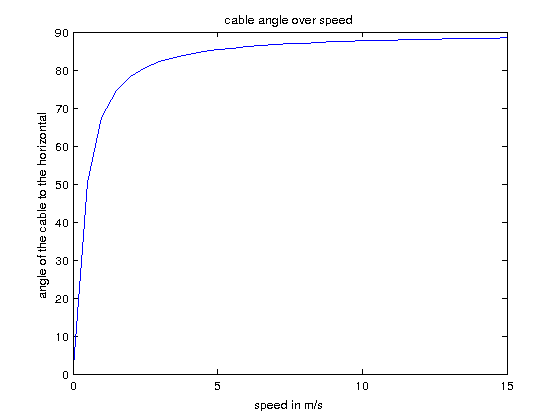
\includegraphics[scale=0.45,angle=0]{inde_cable_angle_speed.png}
    \caption{Angle of the cable when stabilized at the final speed.}
    \label{fig:angleIndSpeed}
    \end{minipage}
    \hfill
    \begin{minipage}[b]{0.45\textwidth}
    \centering
    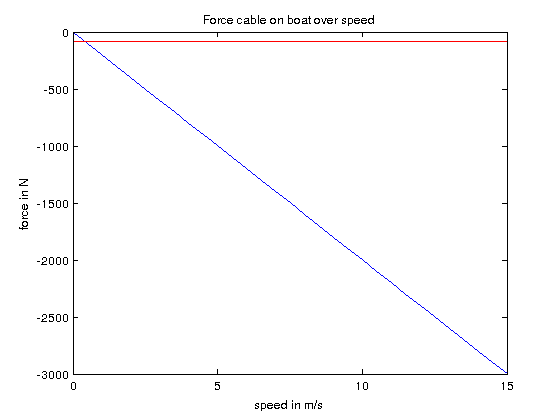
\includegraphics[scale=0.45,angle=0]{inde_cable_force_speed.png}
    \caption{Force of the cable on the boat when stabilized at the final speed.}
    \label{fig:forceIndSpeed}
    \end{minipage}
\end{figure}

By doing simulation with this model, the profile of the angle of the cable over speed is the same as in the Simulink model and the same can be done for the reaction of the cable on the boat, an constant for the vertical reaction and a linear decrease for the horizontal reaction dependant on the fluid friction force.

This model include a tolerance to errors which are resolved by the Baumgarte stabilisation technique but 
there still some left over:


\begin{figure}[H]
\centering
    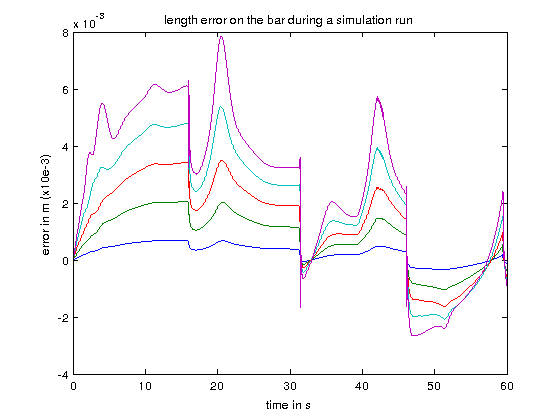
\includegraphics[scale=0.5,angle=0]{error_length_run.png}
    \caption{Error in length of the rods during a simulation run.}
    \label{fig:errorLRod}
\end{figure}

In the figure~\ref{fig:errorLRod} the error in length reach a maximum around one centimetre for a rod length of four meters\footnote{To see simulations : \href{https://www.youtube.com/watch?v=T7DRGq3E5x8}{Fixed cable video} or \href{https://www.youtube.com/watch?v=V4X0PsgsXZY to see simulations}{Moving cable with a constant speed video}}, this error can be considered negligible in this case but in some runs if the start is too sharp then, the simulation may diverge.

In this model each rod can have a different length and mass:

\begin{figure}[H]
\centering
    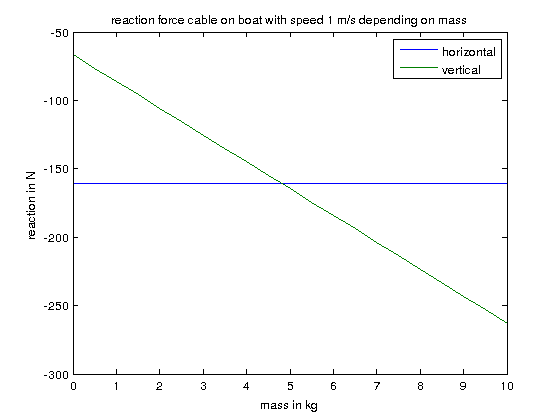
\includegraphics[scale=0.5,angle=0]{inde_cable_force_mass.png}
    \caption{Variation of reaction force of cable on boat depending on mass of last rod.}
    \label{fig:massForce}
\end{figure}

In figure~\ref{fig:massForce} is represented the force of the cable on the boat once stabilized and depending of the mass of the last rod. The horizontal force is constant over mass, this is logical as when stabilized mass does not appear in the horizontal part of the equation \eqref{equ_Stab}. And as for the vertical reaction it vary linearly with the mass,thus corresponding to the precedent equation on the z axis.

Changing the linear mass or the mass of the last rod have different effect on the final angle of the cable(see~\ref{fig:linmassAngle}).

\begin{figure}[H]
\centering
    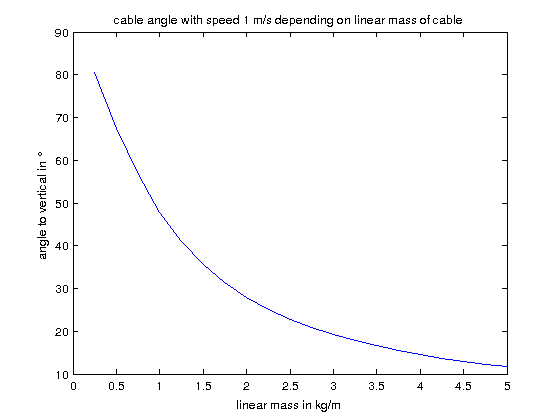
\includegraphics[scale=0.6,angle=0]{inde_cable_angle_linmass.png}
    \caption{Variation of the angle of the cable depending on the linear mass of the rods.}
    \label{fig:linmassAngle}
\end{figure}

To simulate this model there is more than one options, but to not make it diverge tweaking must be made.
If using a fixed-step size integration (Runge-Kutta,ODE45) the step need to be $\sim\mathcal{O}(10^{-3})$, it is the limit of this method and if the cable endure big acceleration it will diverge.

With an solver with variable step-size (ODE23) the result will be in general more accurate but the computation time became very high needing more than one second to compute one second of simulation.If possible Matlab coder should be used to help improve the computation time.
